\section{Régulateur PID}

\subsection{Introduction}

Afin de réguler les variations en sortie $PV$, on utilise un régulateur PID, qui reprend la valeur de $PV$ pour la soustraire à la consigne $SP$ donnant donc l'erreur $E = SP - PV$ à corriger sur $MV$.\\
Pour rappel, un régulateur PID est composé de trois termes:
\begin{itemize}
    \item Le terme proportionnel $P$ qui est proportionnel à l'erreur $E$ et vise une erreur statique nulle.
    \item Le terme intégral $I$ qui est proportionnel à la somme des erreurs passées et donc accumule l'erreur.
    \item Le terme dérivé $D$ qui est proportionnel à la dérivée de l'erreur et vise à corriger anticipativement l'erreur future.
\end{itemize}
La sortie du régulateur est alors donnée par :
\begin{equation}
    MV = K_C \, \left( 1 + \frac{1}{T_I s} + \frac{T_D s}{\alpha T_D s + 1}\right) \, E
\end{equation}

Dans le cadre du laboratoire, le régulateur utilise également le \textbf{Reset de l'Action Intégrale} et la \textbf{Saturation de l'Action Intégrale} venant adapter l'action intégrale en fonction de, respectivement, la valeur de $MV$ en mode manuel, et la saturation de $MV$ atteignant les limites $MV_{MAX}$ / $MV_{MIN}$.
\begin{center}
    $MV_I = MV_{Man} - MV_P - MV_D - MV_{FF}$\\[4pt]
    et\\[4pt]
    $MV_I = MV_{MAX} - MV_P - MV_D - MV_{FF}$
\end{center}

\subsection{Optimisation par la méthode IMC}

Il est important de choisir les paramètres $K_C$, $T_I$ et $T_D$ de façon à implémenter le bon régulateur pour notre processus.
Une façon d'obtenir ces paramètres optimaux est de réaliser un step sur $MV$ et d'observer la dynamique du Processus.
Le modèle trouvé va nous permettre de calculer ces valeurs via des tables.\\
On utilisera la ligne I du tableau présent dans le cours, correspondant à un modèle du second ordre avec délai ($\tau_3 = 0$).
\begin{align*}
    K_C &= \frac{1}{K_P} \, \frac{T_{1p} + T_{2p}}{T_{CLP} + \theta}\\[4pt]
    T_I &= T_{1p} + T_{2p}\\[4pt]
    T_D &= \frac{T_{1p} \, T_{2p}}{T_{1p} + T_{2p}}
\end{align*}
Il est bon de noter que nous aurions pu utiliser la ligne G du tableau (premier ordre avec délai) totalement équivalente étant donné que notre Processus est du premier ordre ($T_{2p} \approx 0$).
La constante $T_D$ et donc l'action Dérivée valant 0, le regulateur devient enfait un régulateur PI.
\begin{align*}
    K_C &= \frac{1}{K_P} \, \frac{T_{1p}}{T_{CLP} + \theta}\\[4pt]
    T_I &= T_{1p}\\[4pt]
    T_D &= 0
\end{align*}
La constante de temps en boucle fermée $T_{CLP}$ est un certain ratio de la première constante de temps du processus $T_{1p}$ définit par $T_{CLP} = \gamma \, T_{1p}$. L'influence de $\gamma$ sera discuté en simulation de boucle fermée par après.

\subsection{Réponse indicielle du régulateur PID}

Nous allons maintenant analyser la réponse du régulateur lorsqu'on applique une erreur $E$ constante à son entrée.
La figure \ref{fig:Step_Response_PID} représente cette réponse.
\begin{figure}[h]
    \centering
    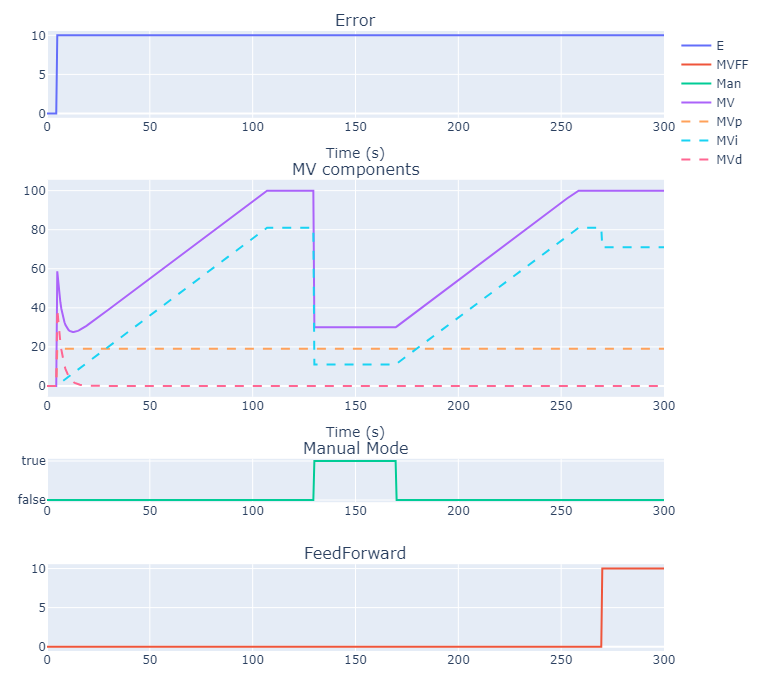
\includegraphics[width=0.8\textwidth]{../Plots/PID/PID_Response_error_step.png}
    \caption{Réponse indicielle du PID à un step sur E}
    \label{fig:Step_Response_PID}
\end{figure}

Premièrement, nous voyons tout au long du graphique que $MV$ est la somme de ces actions $MV = MV_P + MV_I + MV_D + MV_{FF}$.
A l'instant du step sur l'erreur, la composante proportionnelle $MV_P$ augmente instantanément puisqu'elle est proportionnelle à l'erreur, la composante intégrale $MV_I$ est encore nulle puisqu'elle n'a pas encore accumulé d'erreurs, et la composante dérivée $MV_D$ est limitée à $1/\alpha$ puis diminue suivant sa constante de temps $T_D$.

Ensuite, lorsque nous sommes en mode automatique, l'action intégrale $MV_I$ augmente linéairement puisque l'erreur est constante.
Cela va continuer jusqu'à éventuellement atteindre les limites imposées sur la sortie $MV$, ici, une puissance de chauffe $MV_{MAX} = 100\%$ et $MV_{MIN} = 0\%$.
Il est alors nécessaire de réaliser un Reset de l'Action Intégrale, c'est-à-dire, venir adapter la valeur de $MV_I$ pour garder la sortie $MV$ dans les limites.
\begin{equation*}
    MV_I = MV_{MAX} - MV_P - MV_D - MV_{FF}
\end{equation*}

Lorsque l'on passe en mode manuel (boucle ouverte), la valeur de $MV$ est donnée par l'opérateur et donc ici, fixé à 30\%.
En effet, on voit sur le graphe que $MV$ chute à 30\% et que l'action intégrale $MV_I$ est alors adaptée pour garder la sortie $MV$ à cette valeur.

Enfin, une perturbation à été ajoutée à la fin de la simulation pour montrer l'effet de l'action Feed-Forward.
À saturation, le Reset de l'Action Intégrale prends également en compte cette perturbation pour garder la sortie $MV$ dans les limites et donc, on le voit sur le graphe lorsque $MV_I$ est réduit de 10\%.
Si $MV$ ne sature pas, cette perturbation sera directement ajoutée à la sortie $MV$ permettant ainsi de minimiser l'impact sur $PV$.

\subsubsection{Influence de \texorpdfstring{$K_C$}{Kc}}
\begin{figure}[H]
    \centering
    \begin{subfigure}[b]{0.48\textwidth}
        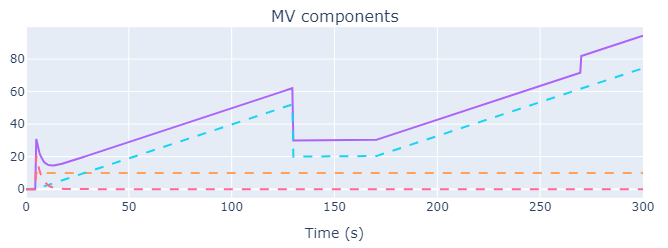
\includegraphics[width=\textwidth]{../Plots/PID/PID_Response_low_Kc.png}
        \caption{$K_C = 1$}
    \end{subfigure}
    \begin{subfigure}[b]{0.48\textwidth}
        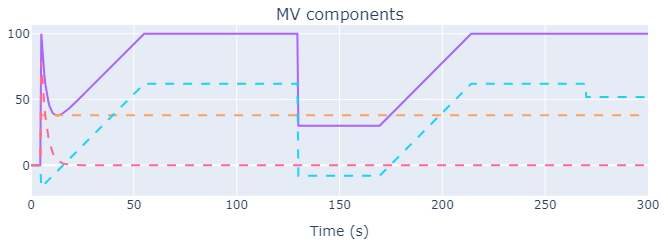
\includegraphics[width=\textwidth]{../Plots/PID/PID_Response_high_Kc.png}
        \caption{$K_C = 3.8$}
    \end{subfigure}
    \caption{Influence de $K_C$ sur la réponse indicielle du PID}
    \label{fig:Kc_Influence_PID}
\end{figure}

\subsubsection{Influence de \texorpdfstring{$T_D$}{Td} et \texorpdfstring{$T_I$}{Ti}}
\begin{figure}[H]
    \centering
    \begin{subfigure}[b]{0.48\textwidth}
        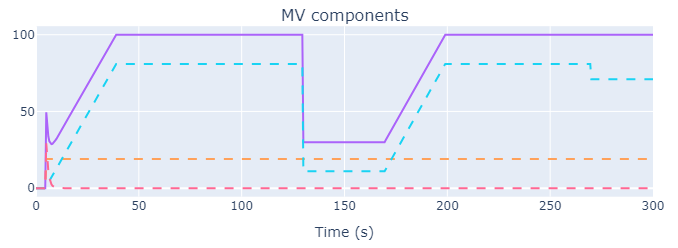
\includegraphics[width=\textwidth]{../Plots/PID/PID_Response_low_Td.png}
        \caption{$T_D = 2\,s$ ($T_I = 8\,s$)}
    \end{subfigure}
    \begin{subfigure}[b]{0.48\textwidth}
        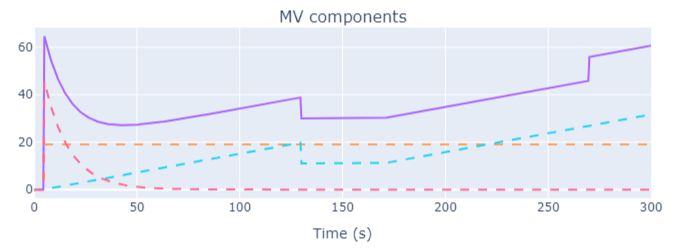
\includegraphics[width=\textwidth]{../Plots/PID/PID_Response_high_Td.png}
        \caption{$T_D = 30\,s$ ($T_I = 120\,s$)}
    \end{subfigure}
    \caption{Influence de $T_D$ et $T_I$ sur la réponse indicielle du PID}
    \label{fig:Td_Influence_PID}
\end{figure}

\subsubsection{Influence de \texorpdfstring{$\alpha$}{alpha}}
\begin{figure}[H]
    \centering
    \begin{subfigure}[b]{0.48\textwidth}
        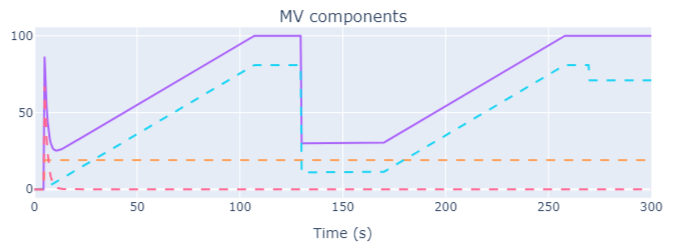
\includegraphics[width=\textwidth]{../Plots/PID/PID_Response_low_alpha.png}
        \caption{$\alpha = 0.2$}
    \end{subfigure}
    \begin{subfigure}[b]{0.48\textwidth}
        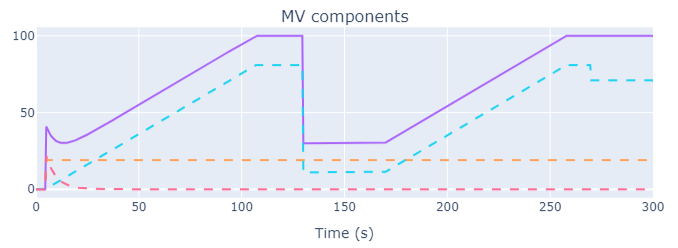
\includegraphics[width=\textwidth]{../Plots/PID/PID_Response_high_alpha.png}
        \caption{$\alpha = 0.8$}
    \end{subfigure}
    \caption{Influence de $\alpha$ sur la réponse indicielle du PID}
    \label{fig:Alpha_Influence_PID}
\end{figure}